\documentclass[main.tex]{subfiles}
\begin{document}

\chapter{Microcontrollore 8051}

\section{Introduzione al microcontrollore 8051}
Il microcontrollore 8051, il primo dei due usati in questo corso, ha una struttura di tipo Harvard. Le sue caratteristiche principali sono riassunte qui di seguito:
\begin{itemize}
    \item memoria programmi distinta da memoria dati e anche doppio bus(uno dedicato alla FLASH e l'altro dedicato alla RAM)
    \item 8bit(celle di memoria a 8 bit ma indirizzamento a 16 bit)
    \item Gestione di interrupt nidificati in ordine di priorità(ma senza l'ausilio di un NVIC (nested vector interrupt controller) dedicato)
    \item Stack da dichiarare(per gestire la chiamata di sottoprogrammi)
    \item Programmazione in Assembly e C 
\end{itemize}

\subsection{Paradigma ad 8 bit}
Il paradigma ad 8 bit è implementato nel seguente modo nell'8051:
\begin{itemize}
    \item Le celle di memoria sono ad 8 bit
    \item La memoria interna RAM è limitata a 256 byte, quindi saranno 256 celle che possono essere indirizzate con soli 8 bit($2^8=256$)
    \item La memoria interna programmi(di tipo flash) essendo indirizzata a 16 bit può arrivare a 64KB, ($2^{16}=65536$ celle di memoria da 1 byte)
\end{itemize}
L'indirizzamento a 16 bit è reso possibile dalla presenza di un latch, il quale in un primo momento, mantenendo alta la sua linea di enable, memorizza la parte alta o \textbf{bassa} dell'indirizzo(prende gli 8 bit, più o meno significativi), poi mantenendo bassa la sua linea, mette a disposizione del bus indirizzi il dato che memorizzato, il quale, insieme agli 8 bit rimanenti forniti dal micro va a formare un indirizzo a 16 bit.

La memoria programmi usata è del tipo FLASH, il che permette di scrivere e cancellare più volte il programma, cosa necessaria durante lo sviluppo. 


\subsection{Configurazione del micro}

Qui di seguito viene riportata la configurazione generica eseguita all'inizio di ogni esperienza con l'8051.

Il primo passo per configurare il microcontrollore è disattivare il watchdog. Per fare ciò viene usato il Configuration Wizard. All'interno di questo software viene creato un file assembly che viene incluso nel progetto del'8051 ed eseguito all'inizio del main mettendo in funzione tutte le periferiche interessate. Un ulteriore step da fare in fase di configurazione è quello di indicare al micro una sorgente esterna per il clock. La sorgente che useremo è un cristallo oscillatore che ha una frequenza di 22.1184 MHz. Questo passaggio è necessario per garantire al micro di avere una frequenza di clock più precisa in quanto quella interna è di ($2\pm0.02$)MHz.
Una volta completata la configurazione nel Wizard, si esporta un file .asm che viene incluso nel progetto e nel file contenente il programma(e.g."led.a51") viene dichiarata una funzione esterna Init\_Device che fa riferimento a quella scritta dal Wizard.

\section{Relazione led}
\subsection{Led in assembly in polling}

In questa esperienza si è programmato il microcontrollore per accende e spegnere il led. Il codice è stato scritto in assembly utilizzando il timer in polling.

Per la realizzazione è necessario impostare la porta P1.6 che controlla l’accensione e lo spegnimento del led, in configurazione push-pull ed impostare il Timer0.
Per realizzare i due cicli su due registri distinti sono stati usati R0 per i cicli che durano un overflow del timer ed R1 per i 10 cicli in cui viene acceso e spento il led. 
Dopo aver configurato il micro, nel main, inizia un loop che dura 10 cicli, all'interno dei quali:
\begin{itemize}
    \item si accende il led
    \item si chiama la funzione timer, all'interno della quale il micro starà per un tempo $\tau$
    \item si spegne il led
    \item si chiama di nuovo timer
    \item si ritorna all'inizio del loop
\end{itemize}
\begin{lstlisting}[caption=Main del programma]
MOV R0, #10
REPEAT:
SETB P1.6 ;accendo il led
LCALL TIMER
CLR P1.6 ;spengo il led
LCALL TIMER
DJNZ R0, REPEAT
\end{lstlisting}
La funzione timer è implementata come una serie di cicli(50), durante i quali:
\begin{itemize}
    \item si aspetta un overflow del timer in un while loop
    \item si resettano le variabili del timer
    \item si controlla se sono passati 50 cicli
\end{itemize}
\begin{lstlisting}[caption=Funzione timer]
TIMER:
	;faccio trascorrere un po' di tempo
	MOV R1, #50 ;voglio che venga eseguito due volte
	FOR:
	SETB TR0 ;faccio partire il cronometro
	WHILE:
		JNB TF0, WHILE ;
	CLR TR0 ; FERMO IL TIMER
	CLR TF0 ;AZZERO IL FLAG DI OVERFLOW
	SETB TR0 ; faccio ripartire il timer
	DJNZ R1, FOR ; loop eseguito 50 volte?
	CLR TR0; fermo il timer
	CLR TF0 ;azzero il flag di overflow
	RET
\end{lstlisting}


\subsection{Led in assembly con interrupt}

La gestione dell'interrupt è il fulcro di questa esperienza. Innanzitutto quindi bisogna abilitarlo nel configuration wizard. È stato poi necessario capire come gestirlo. È stato necessario fare un code segment a 0x000B dove punta l'interrupt del timer0, ovvero la porzione di codice che viene eseguita quando scatta l'interrupt. Visto che lo spazio riservato in 0x000B permette di eseguire solo un'istruzione è necessario fare un JMP ad un'area di memoria programmi in cui è possibile svolgere più istruzioni. In quest'area viene gestito completamente l'interrupt dalle funzioni sotto elencate.

\begin{lstlisting}[caption=Funzione timer]
TIMER:
    CLR TR0; viene fermato il timer
    CLR TF0; si pulisce la flag di overflow
    DJNZ R0, NULLA; si decrementa R0, salta se=0
    JMP SCELTA; questo jump viene eseguito se R0=0

NULLA:
    SETB TR0; faccio ripartire il micro
    RETI; si esce dall'interrupt
\end{lstlisting}
 
 Scelta è una semplice funzione che determina cosa fare, se spegnere oppure accendere il led.
 \begin{lstlisting}[caption=Funzione scelta]
 SCELTA:
	;SE R1 = 1 ALLORA ACCENDO, SE = 0 SPENGO
	MOV A, R1; si sposta nell'acc. R1 per fare l'if
	JZ ACCENSIONE
	JNZ SPEGNIMENTO
 \end{lstlisting}

Mentre le funzioni accensione e spegnimento sono le seguenti
\begin{lstlisting}[caption=Funzioni accensione e spegnimento]
ACCENSIONE:
	SETB P1.6; si accende il led
	MOV R0, #255 ; si imposta R0 a 255
	MOV R1, #1 ; si imposta lo status a R1
	SETB TR0; faccio ripartire il micro
	RETI

SPEGNIMENTO:
	CLR P1.6; si spegne il led
	MOV R0, #255
	MOV R1, #0
	SETB TR0; faccio ripartire il micro
	RETI
\end{lstlisting}
R1 quindi in questo caso è un registro di stato, tiene in memoria lo stato del led, se è acceso o spento.

Ciò che viene eseguito nel main è solamente la configurazione del micro, viene messo in R0 l'indirizzo di 255 e in R1 quello di 0.

\subsection{Led in C}\label{led in C}
Scopo di quest'esperienza è di apprendere l'interazione tra il programma in C e quello in assembly. La parte di configurazione del micro infatti rimane scritta in asm mentre il codice principale è scritto in C. L'interazione in realtà si limita a dichiarare nel file .c una funzione esterna Init Device definita nel file .asm. Il programma in questo caso, invece di limitarsi ad accendere e spegnere il led, permette di regolarne la luminosità tramite il bottone disposto sulla scheda di sviluppo. Dunque le novità del codice rispetto a quelli precedenti sono 
\begin{itemize}
    \item codice in C
    \item gestione della luminosità del led
    \item gesitone dell'interrupt del bottone
\end{itemize}

Quindi andando in ordine il codice in C: volendo operare solo su alcuni bit dei registri di controllo è stato necessario definirli a partire dalle variabili dichiarate nel file C8051f020.h in questo modo:
\begin{lstlisting}
sbit P1_6 = P1 ^ 6;
sbit P3_7 = P3 ^ 7;
\end{lstlisting}
che permette di selezionare solo i bit che ci interessano. 

Per quanto riguarda la luminosità, che in realtà non è regolabile sul micro, viene usato un'escamotage modificando la frequenza con cui viene acceso e spento il led. All'occhio umano il cambio di frequenza di accensione appare come una differente luminosità in quanto la frequenza è paragonabile con il refresh rate dell'occhio. 

La gestione dell'interrupt del bottone viene eseguita in modo molto simile a quella del led, tranne per il fatto che il flag dell'interrupt non è bit addressable quindi per resettarlo è necessario usare una maschera e per il numero di interrupt assegnato. 
Come ulteriore differenza dall'asm infatti si ha che per gestire l'interrupt è necessario definire funzioni il cui nome è seguito da "interrupt" e da un numero che identifica quale interrupt si sta gestendo. 

 Loops identifica quanti cicli di overflow del timer si aspettano prima di cambiare lo stato del led, ovvero identifica la frequenza di accensione e spegnimento. Questo controllo viene effettuato all'interno dell'interrupt del timer.
 \begin{lstlisting}[language=C,caption=Interrupt timer]
 void interruzione_timer(void) interrupt 1{
	//fermo
	TR0=0;
	TF0=0;
	loops--;
	if (loops<=0){
	        //devo cambiare lo stato del led
			if(led_status){
				//accendo
				P1_6=1;
				led_status=0;
				loops=loops_on;
			}
			else{
				//spengo
				P1_6=0;
				led_status=1;
				loops=n_loops-loops_on;
				//faccio ripartire
			}
	}
	TR0=1;
}
 \end{lstlisting}
 
 Dunque si è definita la luminosità come un int che può essere 0, 25,50,75,100. La variabile lumstatus identifica in che stato si è tra i 5 possibili. Essa viene modificata nell'interrupt del bottone, quindi ogni volta che viene schiacciato.
 \begin{lstlisting}[language=C, caption=Interrupt pulsante,label={lst:led in C}]
 void interruzione_pulsante(void) interrupt 19{
	TR0=0;
	TF0=0;
	//cambio status
	if(lum_status<4){
		lum_status++;
	}
	else{
		lum_status=0;
	}
	luminosity=lum_status*25;
	loops_on=n_loops*luminosity/100;
	//resetto tutto
	loops=loops_on;
	led_status=0;
	P1_6=1;
	//reset del flag dell'interrupt esterna 7
	P3IF &= ~0x80;
	TR0=1;//faccio ripartire il timer
}
 \end{lstlisting}

Infine è necessario settare le variabili globali e quelle nel main
\begin{lstlisting}[language=C,caption=Variabili globali]
#define n_loops 5
char idata stack1[16];
int luminosity = 0;
int loops_on;
int loops; //lo stato iniziale=1
int led_status=0;
int lum_status=0;//indica le opzioni(0,25, 50, 75,100)
\end{lstlisting}
\begin{lstlisting}[language=C,caption=main]
SP = (char) (&stack1);
Init_Device();
loops_on=n_loops*luminosity/100;
loops=loops_on;
\end{lstlisting}


%commentare la scelta dello stack

\section{Relazione Seriale}
La comunicazione UART è l'oggetto di questa esperienza. Si è messo in comunicazione il micro con il computer, tramite un cavo che collega la usb del computer con i due pin(più il pin GND) del micro, uno per la trasmissione e uno per la ricezione.

Prima di trasmettere e ricevere un carattere è necessario innanzitutto configurare la UART, con il BAUDE RATE(9600 bps) corretto, e con il timer corretto e infine abilitare l'interrupt.  

Per trasmettere è necessario mettere in SBUF0 il carattere che si vuole mandare, il micro provvederà a trasmetterlo e a trasmissione conclusa genererà un'interrupt settando la flag TI(trasmissione completata). Per quanto riguarda la ricezione invece, il programma entra in interrupt con la flag RI(ricezione completata) dopo aver ricevuto il bit di stop, e mette a disposizione il carattere ricevuto nello SBUF0.  
\subsection{Seriale in C}

In una prima fase del programma il micro trasmetteva un messaggio di benvenuto, nella seconda fase entrava in modalità eco, quindi ad ogni carattere che gli si mandava lui trasmetteva lo stesso carattere. Infine nell'ultima fase memorizzava una serie di caratteri(massimo 10) e dopo un certo carattere("\#") ritrasmetteva la stessa serie. Per realizzare ciò è stata implementata la funzione scelta che a seconda del valore di status(0,1 o 2) svolge compiti diversi. Nella prima trasmette il messaggio a cui punta \textit{puntatore}(nella prima fase è il messaggio di benvenuto ma successivamente diventa il messaggio trasmesso dall'utente al computer), nella seconda viene implementata la modalità eco e nella terza si riceve una serie di caratteri che viene memorizzata in un vettore. Se il messaggio mandato dall'utente è più lungo di 10 caratteri viene trasmesso un messaggio di errore.

\begin{lstlisting}[language=C,caption=Funzione scelta,label={lst:scelta}]
void scelta(void){
	//controllo lo status
	switch(status){
		case(0):
			//trasmetto il messaggio
			i++;
			if (i<lenght_da_trasmettere){
				SBUF0=*(puntatore+i);
			}
			else{
				//ho finito di trasmettere entro in ricezione
				status++;
				i=0;
				REN0=1;
			}
			break;
		case(1):
			key=SBUF0;//ricevo, leggo SBUF0
			RI0=0;
			if(key=='#'){
				i=2;
				status++;
			}
			else{
				if(!loaded){
					loaded=1;
					SBUF0=key;
				}
			}
			break;
		case(2):
			RI0=0;
			if(i<ML+3){
				key=SBUF0;
				//aggiungo il carattere letto al vettore
				msg_ricevuto[i]=key;
				i++;
				if(key=='#'){
					REN0=0; //smetto di ricevere
					status=0;
					puntatore=msg_ricevuto;
					msg_ricevuto[i-1]=CR;
					msg_ricevuto[i]=LF;
					lenght_da_trasmettere=i+1;
					i=0;
					SBUF0=*puntatore;//trasmetto messaggio
				}
			}
			else{
				REN0=0;
				i=0;
				status=0;
				puntatore=msg_errore; //trasmetto errore
				lenght_da_trasmettere=lenght_errore;
				SBUF0=*puntatore;
			}
			break;
	}
}
\end{lstlisting}
La funzione scelta viene chiamata solo dall'interrupt della UART, a prescindere che si sia finito di trasmettere o di ricevere.
\begin{lstlisting}[language=C,caption=Interrupt UART]
void UARTO() interrupt 4{
	if(TI0==1){
		//ho appena finito di trasmettere
		scelta();
		//dice che ha caricato l'ultimo carattere
		loaded=0; 
		//resettare flag
		TI0=0;
		return;
	}
	else if(RI0==1){
		//ho appena finito di ricevere
		scelta();
		return;
	}
	else{
		//ho un problema
		return;
	}
}
\end{lstlisting}

\begin{lstlisting}[language=C, caption=Variabili globali]
#define CR 13
#define LF 10
#define ML 10
uchar key;
uchar idata msg_trsm[]={'C','i','a','o',CR,LF};
uchar lenght_da_trasmettere = 6;
uchar idata msg_errore[]={CR,LF,'E','r',
'r','o','r','e',CR,LF};
uchar lenght_errore=10;
uchar i=0;
uchar * puntatore;
uchar idata msg_ricevuto[ML+4];
uchar status=0;
uchar loaded=0;
\end{lstlisting}
Il tutto inizia trasmettendo il primo carattere del messaggio di benvenuto, una volta che la trasmissione è stata completata si passa al carattere successivo e così via fino alla fine.
Al termine di queste istruzioni il programma entra in un ciclo infinito ed esce solo quando l'utente trasmette dei caratteri, entrando nell'interrupt e quindi nella funzione scelta. 
\begin{lstlisting}[language=C, caption=main]
SP=(char)&stack;
Init_Device();
//inizia trasmissione msg di benvenuto
puntatore = msg_trsm; 
SBUF0=*puntatore;
msg_ricevuto[0]=CR;
msg_ricevuto[1]=LF;
while(1);
\end{lstlisting}
%aggiungere esperienza con oscilloscopio
È stato collegato l'oscilloscopio ai pin dedicata all'UART per controllare il segnale trasmesso. Sono stati ottenuti i seguenti grafici:
\begin{figure}[H]
    \centering
    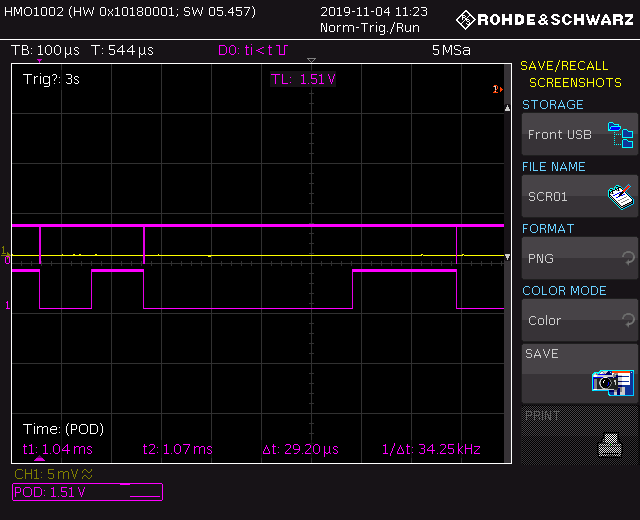
\includegraphics[width=0.7\textwidth]{a_binario.PNG}
    \caption{'a' in binario}
    \label{fig:a}
\end{figure}
\begin{figure}[H]
    \centering
    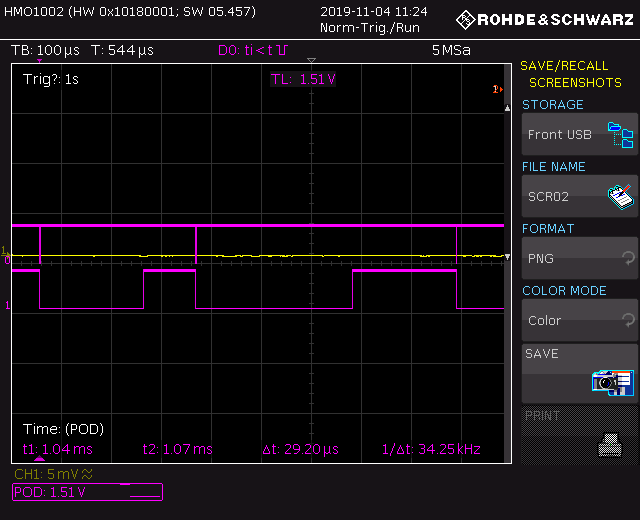
\includegraphics[width=0.7\textwidth]{b_binario.PNG}
    \caption{'b' in binario}
    \label{fig:b}
\end{figure}
\begin{figure}[H]
    \centering
    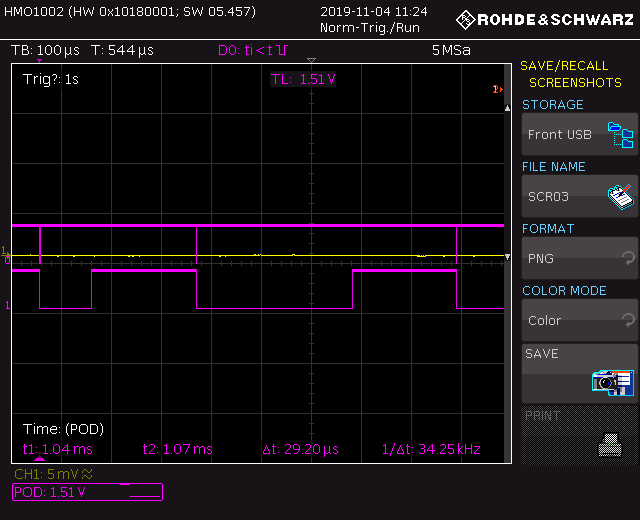
\includegraphics[width=0.7\textwidth]{c_binario.PNG}
    \caption{'c' in binario}
    \label{fig:c}
\end{figure}
I messaggi che sono stati trasmetti dell'Hyperterminal al micro sono 'a', 'b' e 'c', che vengono trasformati in binario(rispettivamente 01100001, 01100010, 01100011), e mandati tramite il pin di trasmissione. Come si puù vedere ci sono i bit di start e quelli di stop.

\subsection{Seriale in assembly}

Questo semplice programma, è una piccola variante di quello precedente in cui si vuole imparare a gestire un vettore in Assembly. Infatti ciò che si definisce è un vettore nella memoria programmi, questo perché il vettore non verrà modificato ma solo letto, contenente il messaggio di benvenuto. L'indirizzo del vettore viene poi passato, subito dopo la configurazione del micro, al Data Pointer. Viene successivamente implementata una funione NEXT che salva nell'Accumulator il carattere successivo in modo tale che sia accessibile dal main del programma in c. Dunque nel programma in C basterà chiamare questa funzione e prendere il carattere contenuto in A e trasmetterlo. 


\begin{minipage}{0.49\textwidth}
\begin{lstlisting}[caption=Vettore in Assembly]
VETTORE SEGMENT CODE
STACK SEGMENT IDATA
NEXT SEGMENT CODE
RSEG STACK
STACK2: DS 10H
RSEG VETTORE
VETT: DB 'Ciao',00H
RSEG NEXT
N:	MOVC A,@A+DPTR
    RET
RSEG CODICE
START:
	LCALL Init_Device
	MOV DPTR, #VETT
	RET
END
\end{lstlisting}
\end{minipage}%
\hfill
\begin{minipage}{0.49\textwidth}
\begin{tabular}{|p{0.8\textwidth}}
\begin{lstlisting}[caption=codice in C]
NEXT();
*puntatore=
(uchar)ACC;
\end{lstlisting}
\end{tabular}
\end{minipage}%

\end{document}
